%!TEX root = ../../14-icra-RealTimeNMPC.tex

\tikzstyle{block} = [draw, fill=blue!20, rectangle,
    minimum height=2em, minimum width=5em, align=center]
\tikzstyle{sum} = [draw, fill=purple, circle, node distance=1cm]
\tikzstyle{input} = [coordinate]
\tikzstyle{output} = [coordinate]
\tikzstyle{pinstyle} = [pin edge={to-,thin,black}]

% The block diagram code is probably more verbose than necessary
\footnotesize
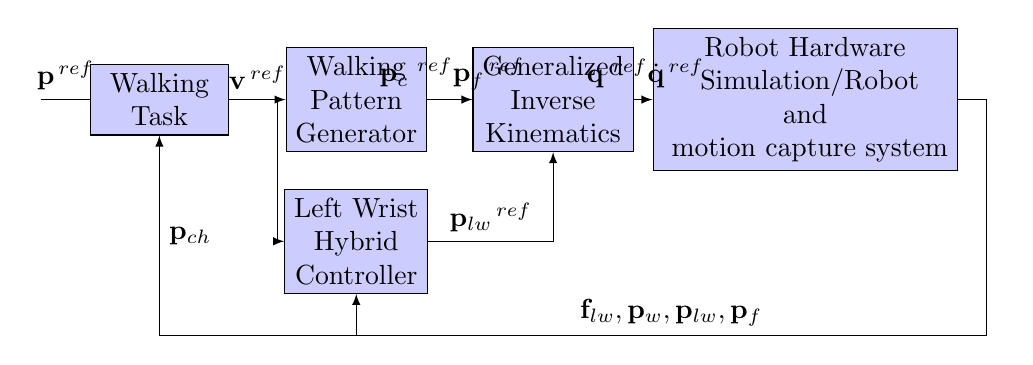
\begin{tikzpicture}[auto, node distance=2cm,>=latex]
    % We start by placing the blocks
    \node [input]  at (0.0, 0.0) (input)  {};
    \node [input]  at (3, 0.0) (velocity) {};
    \node [input]  at (5.5, -1.0) (feedback)  {};
    \node [input]  at (12, -3.0) (feedback2)  {};
    \node []    at ( 0.0, 0.0) (sumin)  {};
    %\node [output]    at ( 15, 0.0) (sumout) {};

    \node [block] at (4,-1.8) (lwc) {
        Left Wrist\\
        Hybrid\\
        Controller        
    };

    \node [block] at (1.5,0.0) (walking) {
        Walking \\
        Task    
    };

    \node [block] at (4,0) (wpg) {
         Walking\\
         Pattern\\
         Generator
    };
%    \node [block] at (4.2,0) (dyn) {
%        Dynamic\\
%        Filter
%    };
    \node [block] at (6.5,0) (sot) {
         Generalized\\
         Inverse\\
         Kinematics
    };
    \node [block] at (9.7, 0) (system) {
    		 Robot Hardware\\
    		{ Simulation/Robot}\\
    		and\\
    		{ motion capture system}
    	};

    % PATHS
    	% Forward chaine
    \draw [draw,-] (input) -- node { ${\mathbf{p}}^{\,{\text {ref}}}$} (walking);
    
    \draw [draw,->] (walking) -- node { ${\mathbf v}^{\,{\text{ref}}}$} (wpg);
%    \draw [draw,- ] (walking) -- node {} (velocity);
    \draw [draw,->] (velocity) |- node {} (lwc);
%    \draw [->] (wpg) -- node { $c^{ref},f^{ref}$} (dyn);
%    \draw [->] (dyn) -- node { $\tilde{c}^{\,ref},f^{ref}$} (sot);
    \draw [->] (wpg) -- node { $
    \begin{matrix}
    {\mathbf{p}_c}^{\,{\text {ref}}} \\
     {\mathbf{p}_f}^{\,{\text {ref}}}
    \end{matrix}        
    $} (sot);
    \draw [->] (sot) -- node { $
    \begin{matrix}
    {\mathbf q}^{\,{\text{ref}}}\\
    \dot{{\mathbf q}}^{\,{\text{ref}}}
    \end{matrix}        
    $} (system);
    
    \draw [->] (lwc) -| node [near start, above]{ ${\mathbf{p}_{lw}}^{\,{\text {ref}}}$} (sot);
    %\draw [->] (system) -- node {} (sumout);

    % Feedback chaine
%    \draw [- ] (dyn)      -| node {} (feedback);
%    \draw [->] (feedback) -| node {} (wpg);
    
    \draw [- ] (system)    -| node {} (feedback2);
    \draw [->] (feedback2) -| node [near start, above]{ $\mathbf{f}_{lw},\mathbf{p}_{w},\mathbf{p}_{lw},\mathbf{p}_{f}$} (lwc);
    \draw [->] (feedback2) -| node [near end, right]{ $\mathbf{p}_{ch}$} (walking);

%    \draw [->] (dyn) -| node[above right] { $\hat{c}^{\,x,y,\theta}$, $\hat{f}^{\,\,x,y,\theta}$} (wpg);
\end{tikzpicture}
%\caption{This scheme describe the feedback loop used to control the humanoid robot HRP-$2$. With ${\mathbf{p}}^{\,{\text {ref}}}$ as the user defined pose, ${\mathbf{v}}^{\,{\text {ref}}}$ as the velocity computed from the walking task, ${\mathbf{p}_c}^{\,{\text {ref}}}$ as the center of mass reference trajectory, ${\mathbf{p}_f}^{\,{\text {ref}}}$ as the feet reference trajectories, ${\mathbf q}^{\,{\text{ref}}},\dot{{\mathbf q}}^{\,{\text{ref}}}$ being respectively the generalized position and velocity vector, ${\mathbf{p}_{lw}}^{\,{\text {ref}}}$ as the reference left wrist position, $\mathbf{f}_{lw},\mathbf{p}_{w},\mathbf{p}_{lw},\mathbf{p}_{f},\mathbf{p}_{ch}$ being respectively the measures of the left wrist force sensor, the waist position, the left wrist position, the feet position and the chest position.}
